\documentclass{article}
\usepackage[utf8]{inputenc}
\usepackage{ngerman}                            % Beschriftungen auf Deutsch
\usepackage{hyperref}                           % URLs benutzen
\usepackage{listings}                           % Code Formatierung
\usepackage{xcolor}                             % Farben für Code
\usepackage[toc, section=section]{glossaries}   % Glossar
\usepackage{pdfpages}                           % PDF anzeigen

\title{InformatiCup - Team Stream}
\author{Christoph Schnell \and Jasper Lorenz \and Robin Schmöcker}
\date{Oktober 2019 - Januar 2020}

\renewcommand{\familydefault}{\sfdefault} % Sans-serif benutzen

\newcommand{\fullref}[1]{\hyperref[{#1}]{\ref{#1} \nameref{#1}}} % Klickbare Links mit Nummer und Name

\newcommand{\faqentry}[2]{\noindent\textbf{Q:} #1\newline\newline\textbf{A:} #2\newline\newline\newline} % Schönes FAQ

\newcommand{\gquote}[1]{\glqq #1\grqq} % Deutsche Anführungszeichen

% Credits to some guy on stack overflow
\newcommand{\displayimage}[1]{\begin{center}\makebox[\textwidth]{\includegraphics[width=\textwidth]{#1}}\end{center}}


% Credits to another guy on stack overflow
\makeatletter % Short minus in lstlisting
\lst@CCPutMacro
    \lst@ProcessOther {"2D}{\lst@ttfamily{-{}}{-}}
    \@empty\z@\@empty
\makeatother

\let\oldgls\gls
\renewcommand{\gls}[1]{\emph{\oldgls{#1}}} % Kursive Glossar Einträge

\lstset{
    basicstyle=\tiny,
    columns=fullflexible,
    tabsize=4,
    rulecolor=\color{black},
    numbers=left,
    keywordstyle=\color{purple},
    frame=single,
    language=Java
}

\makeglossaries {

\newglossaryentry{aktives Pathogen}{
    name=aktives Pathogen,
    description={Siehe \fullref{sec:AktivesPathogen}}
}

\newglossaryentry{starkes Pathogen} {
    name=starkes Pathogen,
    description={Siehe \fullref{sec:StarkesPathogen}}
}

\newglossaryentry{langsames Pathogen}{
    name=langsames Pathogen,
    description={Siehe \fullref{sec:LangsamesPathogen}}
}

\newglossaryentry{schnelles Pathogen}{
    name=schnelles Pathogen,
    description={Siehe \fullref{sec:SchnellesPathogen}}
}

\newglossaryentry{ignoriertes Pathogen}{
    name=ignoriertes Pathogen,
    description= {Siehe \fullref{sec:IgnoriertesPathogen}}
}
 
\newglossaryentry{GI Client} {
    name=GI Client,
    description={Kommandozeilenwerkzeug der Gesellschaft für Informatik, zu finden unter \url{https://github.com/informatiCup/informatiCup2020/releases}}
}
}

\begin{document}
\maketitle
\tableofcontents

\newpage
\section{Einleitung}
\subsection{Vorwort}
Wenn eine Pandemie die Menschheit auszulöschen droht, dann braucht die Welt Mut, Stärke, Intelligenz, Weisheit und Geschick. Anders gesagt es braucht die Besten der Besten. Die F.L. Bauern unter den Softwareingenieuren. Die Turinge unter den Programmierern. Die Admiral Trips unter den Pathogenen. Eben die \gquote{Crème de la Crème}. Die Welt hat Glück, denn eine Gruppe junger Programmierer vereint genau diese Eigenschaften: Team Stream. \\
Ohne weitere Selbstbeweihräucherung nun zur Dokumentation, welche sich grob wie folgt gliedert. Zunächst wird erläutert, wie unsere Lösung zu installieren und im nachfolgenden Kapitel auch zu bedienen ist. Auf die grafische Oberfläche wird genauer eingegangen. Anschließend wird der theoretische Lösungsansatz dargelegt, der vielleicht erfrischenderweise mal kein neuronales Netz beinhaltet. Bevor die Umsetzung des Lösungsansatzes im Code im Detail beschrieben wird, wird die Software Architektur erläutert. Danach wird erklärt wie unser Programm weiterzuentwickeln ist und welche Schritte wir unternommen haben, um die Stärke unseres Programmes zu beweisen. \\
Zum Ende hin wird kurz reflektiert, was in dieser finalen Abgabe nicht optimal lief, bzw. was wir beim nächsten mal anders  machen würden. Zum Schluss werden noch häufig gestellte Fragen zu unserem Projekt beantwortet und Daten dargelegt, die wir über die Spielversion des bereitgestellten Kommandozeilenwerkzeugs gefunden haben.

\subsection{Schnellstart}
\label{sec:Schnellstart}
Die schnellste und einfacheste Weise den \gls{GI Client} zu testen ist über den von uns bei AWS bereitgestellten Webservice. Um diesen nutzen zu können, muss der \gls{GI Client} mit dem \gquote{-u} Parameter und folglich der URL unseres Webservices aufgerufen werden. \\
Dies sieht z.B. unter Linux wie folgt aus.
\begin{lstlisting}[language=bash, basicstyle=\footnotesize, numbers=none]
\$ ./ic20_linux -u https://udi8pt9vo9.execute-api.us-east-1.amazonaws.com/default/
\end{lstlisting}
\newpage

\section{Installation}
Dieses Kapitel erklärt die Installation unseres Webservices. Möchte man unseren Webservice ohne Installation nutzen, so können die Schritte unter \fullref{sec:Schnellstart} befolgt werden.
\subsection{Bauen der Jar Datei}
\label{sec:JarBuild}
Sowohl für \fullref{sec:LokalerBuild}, als auch für \fullref{sec:AWSBuild}, muss zuerst die Jar Datei von unserem Projekt gebaut werden. Dazu muss die Oracle Java Version 8 und Maven installiert sein. Zum leichteren Herunterladen von Git-Hub sollte auch noch Git installiert sein. Sind diese Grundlagen geschaffen, gilt es als erstes das Git-Repository zu clonen. Alternativ kann das Projekt auch als Zip-Datei von Git-Hub heruntergeladen und entpackt werden.
Hier wird ein Beispiel für das Clonen mit HTTPS gezeigt.
\begin{lstlisting}[language=bash, basicstyle=\footnotesize, numbers=none]
  \$ git clone https://github.com/jasZnerol/InformatiCup2020.git
\end{lstlisting}
Es sollte nun ein neuer Ordner namens \gquote{informatiCup2020} vorhanden sein. In diesen muss man nun wechseln.
\begin{lstlisting}[language=bash, basicstyle=\footnotesize, numbers=none]
  \$ cd informaticup2020/
\end{lstlisting}
Zum Bauen muss folgender Maven-Aufruf aus dem Root-Verzeichnis des Projektes erfolgen.
\begin{lstlisting}[language=bash, basicstyle=\footnotesize, numbers=none]
  \$ mvn package
\end{lstlisting}
Die Jar-Datei sollte nun in dem Unterordner \gquote{target} liegen und \gquote{ic\_webservice-20.jar} heißen.

\subsection{Lokale Version mit GUI}
\label{sec:LokalerBuild}
Um unser Programm lokal auszuführen, muss Oracle Java 8 installiert sein. Wurden die Schritte von \fullref{sec:JarBuild} befolgt so muss nur folgender Befehl zum Ausführen des
Programms aufgerufen werden.
\begin{lstlisting}[language=bash, basicstyle=\footnotesize, numbers=none]
  \$ java -jar target/ic_webservice-20.jar
\end{lstlisting}
War die Installation erfolgreich, so sollte sich an dieser Stelle die zur lokalen Version gehörende, GUI öffnen. Mehr Informationen finden sich unter \fullref{sec:GuiNutzung}. \\
Da die Aufgabenstellung einen Befehl zum Bauen und Ausführen vorgibt, können die Befehle auch kombiniert werden.
\begin{lstlisting}[language=bash, basicstyle=\footnotesize, numbers=none]
  \$ mvn package && java -jar target/ic_webservice-20.jar
\end{lstlisting}
\newpage

\subsection{Bereitstellung bei AWS}
\label{sec:AWSBuild}
Wurden die Schritte von \fullref{sec:JarBuild} befolgt, gilt es die gebaute Jar bei AWS als Lambda-Funktion bereitzustellen. Dafür öffnet man die AWS-Konsole unter der folgenden URL:
\begin{center}
    \url{https://console.aws.amazon.com/console/home}
\end{center}
Als erstes sucht man in der Suchleiste nach \gquote{Lambda}.
\displayimage{resources/aws_installation/search_lambda.png}
Dannach erstellt man eine neue Lambda-Funktion.
\displayimage{resources/aws_installation/create_function.png}
Nun gilt es die Optionen zum Erstellen festzulegen. Dabei wählen wir \gquote{Author from scratch}, einen beliebigen Namen und Java 8 als Laufzeit Umgebung.
\displayimage{resources/aws_installation/create_function_detail.png}
Jetzt muss ein Auslöser zur Funktion hinzugefügt werden.
\displayimage{resources/aws_installation/add_trigger.png}
Wir wollen eine neu erstellte API als Auslöser wählen. Darum wählen wir als Auslöser das \gquote{API Gateway}.
\displayimage{resources/aws_installation/select_api_gateway2.png}
Danach direkt \gquote{Create new API}.
\displayimage{resources/aws_installation/create_new_api.png}
Die zu erstellende API soll eine Rest-API sein. Als Sicherheitseinstellung wählen wir \gquote{öffentlich}.
\displayimage{resources/aws_installation/rest_api.png}
Damit die Lambda-Funktion noch unseren Code ausführt, muss jetzt die gebaute Jar noch hochgeladen werden.
Dafür wählt man \gquote{Upload}. Nachdem die gebaute Jar aus dem target Ordner hochgeladen wurde, muss noch ein AWS-Handler festgelegt werden.
Dieser ist in unserem HTTP-Package zu finden. Der Handler wird auf \gquote{app.http.AWSHandler::handleRequest} gesetzt.
\displayimage{resources/aws_installation/upload_jar.png}
Die Einstellung muss man nun noch speichern und dann ist das Bereitstellen auf AWS fast abgeschlossen. Die URL des neuen Webservice findet sich unter der Rest-Api als \gquote{endpoint}.
\displayimage{resources/aws_installation/find_endpoint.png}
Um die Ausführung zu gewährleisten, muss eine weitere Einstellung der API geändert werden. Dazu suchen wir zuerst die API in der AWS-Konsole.
\displayimage{resources/aws_installation/select_api_gateway.png}
Wir wählen unsere gerade erstellte API.
\displayimage{resources/aws_installation/select_our_api.png}
Danach muss \gquote{Any} ausgewählt werden.
\begin{center}
    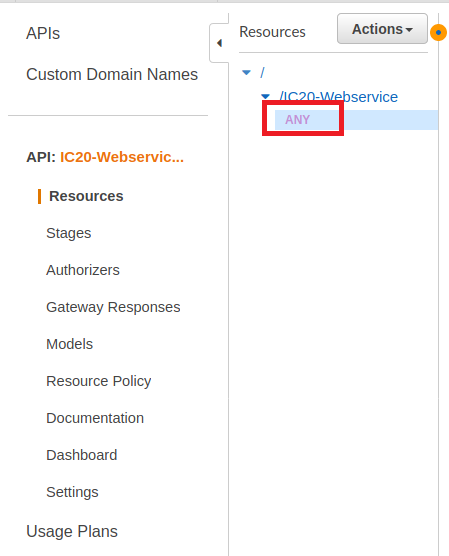
\includegraphics[scale=0.7]{resources/aws_installation/select_any.png}
\end{center}
Anschließend die Integrationsanforderung.
\displayimage{resources/aws_installation/select_integration.png}
Nun muss die Checkbox Lambda-Proxy \textbf{deaktiviert} werden.
\displayimage{resources/aws_installation/select_proxy.png}
Um die Änderungen Wirksam zu machen, muss die API neu bereitgestellt werden. Dazu wählt man erst Aktionen aus und in dem Drop-Down-Menu \gquote{bereitstellen}.
\begin{center}
    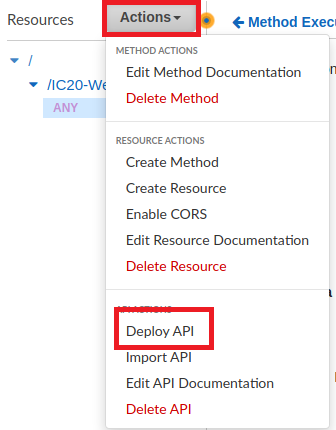
\includegraphics[scale=0.7]{resources/aws_installation/select_deploy.png}
\end{center}
Als nächstes wählt man die Stufe \gquote{default} und stellt sie bereit.
\displayimage{resources/aws_installation/select_default.png}
Nachdem die Einstellung gespeichert ist, kann die API genutzt werden.
\displayimage{resources/aws_installation/select_save.png}
Will man nun den \gls{GI Client} zum neuen Webservice aufrufen, geht das (z.B. unter Linux) wie folgt.
\begin{lstlisting}[language=bash, basicstyle=\footnotesize, numbers=none]
 \$ ./ic20_linux -u <API endpoint>
\end{lstlisting}

\newpage
\section{Benutzung}
\subsection{Benutzung über AWS}
Die Benutzung des bei AWS deployten Webservices entspricht der Beschreibung unter \fullref{sec:Schnellstart}. Sollte man das Programm selber deployt haben, muss lediglich die URL des eigenen Webservices verwendet werden.

\subsection{Benutzung der lokalen Version}
\label{sec:GuiNutzung}
Nachdem die Installationsanleitung unter \fullref{sec:JarBuild} befolgt wurde, lässt sich unser Programm mit folgendem Befehl lokal ausführen.
\begin{lstlisting}[language=bash, basicstyle=\footnotesize, numbers=none]
  \$ java -jar target/ic_webservice-20.jar
\end{lstlisting}
\subsubsection{Benutzung der graphischen Oberfläche}
Man kann nun ein Spiel schrittweise automatisch, sowie selber manuell spielen. \\
Ein blauer Ausgabetext gibt dabei Informationen über den aktuellen Zustand an. Startet man an dieser Stelle den \gls{GI Client}, so sollte der Text ausgegeben werden, dass ein Spiel stattgefunden hat.
Nun kann man durch den \gquote{Auto turn} Knopf einen Zug von der Heuristik ausführen lassen. Optional lässt sich im Textfeld \gquote{amount} eine gewisse Anzahl von automatischen Zügen angeben. \\
Die Tooltips geben hierbei weitere Informationen darüber an, was welche Knöpfe machen und welche Informationen zum Ausführen der Aktion gebraucht werden.

\subsubsection{Benutzung ohne graphische Oberfläche}
Bekommt der Server mehr als eine Anfrage gleichzeitig oder wird das GUI über das rote X geschlossen, so schließt sich das GUI und der Server wechselt in einen Modus, in dem alle Anfragen mit unserer Heuristik beantwortet werden. Alle weiteren einkommenden Spiele, sowie das Spiel, welches derzeit in der GUI war, wird mit unserer Heuristik gespielt.
\subsubsection{Beenden des Servers}
Im GUI lässt sich der Sever über den \gquote{Quit} Knopf beenden.\\
Wurde der Server im Hintergrund gestartet, und das GUI ist nicht mehr offen, so kann der Server mit einer einfachen Anfrage an localhost:50123 beendet werden, solange diese nicht vom Typ Post ist. Dazu kann beispielsweise im Browser localhost:50123 in das Adressfeld eingegeben werden.
\subsubsection{Anzeige der Fehlermeldungen des Webservices}
Da Fehlermeldungen über \gquote{stderr} ausgegeben werden, muss der Webservice über eine Kommandozeile/Bash gestartet werden damit diese angezeigt werden. Startet man ihn über einen Doppelklick auf die Jar Datei so kann man sie nicht sehen.
\subsection{Benutzung des Testskripts}
\label{sec:TestskriptNutzung}
Das Testskript, welches als Test.py im Wurzelverzeichnis unseres Projekts liegt, bietet verschiedene Arten die lokale als auch die von uns deployte Version zu testen. Testen heißt in dem Fall, dass man beliebig viele Spiele, auch parallel, spielt und eine Ausgabe über die aktuelle Winrate erhält. Um es zu benutzen, muss Python Version 3 installiert sein. Es funktioniert sowohl auf Windows, als auch auf Linux. Vor der Nutzung muss der \gls{GI Client} in den gleichen Ordner des Test Skripts gelegt werden.\\
Um sich alle Möglichkeiten, um das Skript auszuführen, von dem Skript selber ausgeben zu lassen, führt man das Skript mit der Flag \gquote{-h} oder \gquote{--help} aus.
\begin{lstlisting}[language=bash, basicstyle=\footnotesize, numbers=none]
  \$ python3 Test.py -h
\end{lstlisting}
Führt man das Skript ohne zusätzliche Flags aus, werden die ersten 100 Seeds, in 4 Threads, über den lokalen Webservice auf localhost:50123 gespielt. Dem entsprechend muss dieser gestartet sein. Wie man diesen startet, findet sich unter \fullref{sec:LokalerBuild}. \\
Will man den deployten Webservice testen, fügt man die Flag \gquote{-aws} hinzu.
\begin{lstlisting}[language=bash, basicstyle=\footnotesize, numbers=none]
  \$ python3 Test.py -aws
\end{lstlisting}
Sollte man die Anzahl der Threads, also die Anzahl der gleichzeitig laufenden Spiele ändern wollen, fügt man die Flag --threads \%AnzahlDerThreads hinzu.
\begin{lstlisting}[language=bash, basicstyle=\footnotesize, numbers=none]
  \$ python3 Test.py --threads 10
\end{lstlisting}
Wenn man Spielseeds aus einem bestimmten Bereich (z.B. von 1 bis 1000) spielen will, so fügt man die Flag --range \%Start \%Ende hinzu.
\begin{lstlisting}[language=bash, basicstyle=\footnotesize, numbers=none]
  \$ python3 Test.py --range 1 1000
\end{lstlisting}
Zusätzlich ist es möglich Seeds in einer Datei anzugeben. Diese Datei muss im gleichen Ordner wie Test.py liegen und seeds.txt heißen. Die Seeds müssen zeilenweise in der Datei liegen.
Durch das Hinzufügen der flag \gquote{-file} werden die Seeds aus der Datei genutzt. Gibt man zu dieser Flag noch eine \gquote{range} an, so wird diese ignoriert.
\begin{lstlisting}[language=bash, basicstyle=\footnotesize, numbers=none]
  \$ python3 Test.py -file
\end{lstlisting}
Da unsere Heuristik für Aktionen mit gleichen Wert nicht deterministisch ist und der \gls{GI Client} einen gewissen Zufallsfaktor beinhaltet, lässt sich die Flag \gquote{-consistency} hinzufügen, welche fortlaufend die gleichen Seeds spielt, damit sich diese vergleichen lassen. Will man z.B. die Einheitlichkeit der Winrate zwischen den Seeds 60 und 70 testen, sieht der Aufruf folgendermaßen aus.
\begin{lstlisting}[language=bash, basicstyle=\footnotesize, numbers=none]
  \$ python3 Test.py -consistency --range 60 70
\end{lstlisting}
Die Flags lassen sich beliebig kombinieren. So kann man z.B. den deployten Webservice auf folgende Weise effizient auf eine konsistente Winrate für die ersten 1000 Seeds testen.
\begin{lstlisting}[language=bash, basicstyle=\footnotesize, numbers=none]
  \$ python3 Test.py -aws -consistency --threads 8 --range 1 1000
\end{lstlisting}
\newpage

\section{Lösungsidee}
\subsection{Entwicklung von Ideen}
Um ein Gefühl für das Spiel zu bekommen, haben wir die GUI entwickelt. Diese ermöglichte es uns Spiele selber zu spielen und das Verhalten der Pathogene genauer kennenzulernen. \\
Außerdem haben wir ein Skript geschrieben, welches uns alle Informationen über sämtliche Städte und alle gefundenen Pathogene in den ersten 436 Seeds liefert. Zeitgleich haben wir dadurch eine Sammlung der Seeds erstellt, welche es uns ermöglichte fast beliebige Startzustände zum selbstständigen Testen unserer Heurisitik zu wählen. Die Liste mit den Seeds findet sich unter \fullref{sec:Anhang}\\
Um mit diesem Grundgerüst an Informationen und Möglichkeiten effiziente Wege zum Bekämpfen der Pathogene zu finden, begann die Entwicklung der Heuristik. \\
Die Lösungsidee der finalen Lösung ist eine lineare Auswertung aller möglichen Aktionen. Dies findet nach jeder ausgeführten Aktion erneut statt. \\
Die Heuristik basiert dabei auf einzelnen Ideen, die inkrementell hinzugefügt wurden. Ob eine Verbesserung vorliegt, wurde ständig mit unserem Winrate-Testskript überprüft. Man könnte also von \gquote{Winrate driven Development} sprechen. Das soll heißen, dass zunächst die einfachsten Ideen implementiert wurden, wie z.B. \fullref{QuarantaeneSchutz} zum Schutz der restlichen Weltbevölkerung. Häufig entstanden Ideen aus Problemsituation von einzelnen Seeds. Z.B. Seed 4 und \fullref{QuarantaeneSchutz} zum Schutz der Bevölkerung der Stadt unter Quarantäne. \\ Funktionierte nun eine Idee für diesen einen Seed, so konnte man sie für mehrere Spiele mit dem erstellten Testskript testen. Eine nützliche Idee sollte minimale Verbesserungen an der Winrate hervorheben.
War dieser abschließende Test erfolgreich, wurde der Prozess mit der nächsten Idee fortgesetzt. \\\\
Dabei ist der größte Aufwand das Entwickeln der Ideen und das Finden von typischen Problemsituationen. Eine Vorgehensweise, welche das Finden von Problemsituationen ermöglichte, war das Testen von mehreren Seeds und das anschließende manuelle Spielen von verlorenen Seeds. 
Konnte man den Seed auf einfache Weise manuell gewinnen galt es zu vergleichen, was die Heuristik anders tat als man selber und diese Idee anschließend umzusetzen. \\ 
Dabei stellte sich schnell ein Problem heraus. Durch das Wählen anderer Aktionen wird der folgende Spielablauf massiv verändert, da die Aktionen den internen Zufallsgenerator des \gls{GI Client}s beeinflussen. \\\\
Insgesamt ist es uns so gelungen eine effektive Heuristik zu entwickeln und ein umfassendes Verständnis für den internen Speilablauf des \gls{GI Client} zu entwickeln. Wobei es dennoch einige ungeklärte Fragen gibt, z.B. was die \gquote{globalen Events}, wie z.B. \gquote{largeScalePanic} konkret bewirken.
\newpage

\subsection{Verworfene Ansätze}
Zunächst erschien die Aufgabe wie ein größeres Rucksackproblem. Jede Aktion kostet eine gewisse Anzahl an Punkten, bringt aber auch einen bestimmten Wert mit sich. Es gilt also die Menge an Aktionen mit maximalem Wert zu finden. Dies stellte sich aber schnell als problematisch heraus. Eine Lösung für das Rucksackproblem ist eine Menge von Aktionen. Problematisch ist es nun eine solche Menge aufgrund möglicher Abhängigkeiten der Aktionen untereinander zu bewerten. Ein Beispiel ist eine Menge, die nur die Aktionen \gquote{Medikament entwickeln} und \gquote{Impfstoff entwickeln} enthält. Hier ist der Wert der Menge nicht die Summe der beiden Aktionen, da es weniger wertvoll ist ein Medikament zu entwickeln, wenn bereits ein Impfstoff entwickelt wird, oder vice versa.
\label{sec:Ansaetze}
\subsection{Umsetzung der Gesamtidee}
Um eine möglichst gute Aktion zu ermitteln, wird jeder möglichen Aktion eine Wertung zugewiesen. Um die beste Aktion zu ermitteln, werden alle Aktionen verglichen und die Aktion mit der größten Wertung wird ausgewählt. Hierbei befinden sich die Wertungen nicht in einer gleichmäßig verteilten Größenordnung. Weiterhin werden viele Aktionen ausgeschlossen indem sie null Punkte bekommen.
\subsection{Pathogen Klassifikationen}
Um Pathogene allgemein beurteilen zu können, werden die Pathogene anhand ihrer Eigenschaften klassifiziert und in Gruppen zusammengefasst.
\subsubsection{Aktives Pathogen}
\label{sec:AktivesPathogen}
Global gesehen ist ein aktives Pathogen ein Pathogen, welches noch mindestens eine Stadt infiziert hat. Lokal gesehen ist ein aktives Pathogen ein Pathogen, welches die betrachtete Stadt infiziert hat.
\subsubsection{Starkes Pathogen}
\label{sec:StarkesPathogen}
Ein starkes Pathogen tötet innerhalb so weniger Runden die Hälfte der Weltbevölkerung, dass das Entwickeln von Medikamenten oder Impfstoffen zu lange dauert, um eine Niederlage zu verhindern. Um als starkes Pathogen klassifiziert zu werden, muss das Produkt der numerischen Repräsentation der Werte für \gquote{Infectivity}, \gquote{Lethality}, 6 - \gquote{Duration} und \gquote{Mobility} größer oder gleich 220 sein. \\
Die Implementierung zum erkennen von starken Pathogenen findet sich in der Methode \gquote{doQuarantine} unter \fullref{code:DoQuarantine}.
\subsubsection{Langsames Pathogen}
\label{sec:LangsamesPathogen}
Ein langsames Pathogen infiziert langsam Städte und ihre Bevölkerung. Um als langsames Pathogen klassifiziert zu werden, muss das Produkt der numerischen Repräsentation der Werte für \gquote{Infectivity} und \gquote{Mobility} kleiner oder gleich 6 sein.\\
Die Implementierung zum Erkennen von langsamen Pathogenen befindet sich in der Methode \gquote{doDevVaccine} unter \fullref{code:DoDevVaccine}.
\subsubsection{Schnelles Pathogen}
\label{sec:SchnellesPathogen}
Ein schnelles Pathogen infiziert schnell viele Städte und ihre Bevölkerung. Um als schnelles Pathogen klassifiziert zu werden, muss das Produkt der numerischen Repräsentation der Werte für \gquote{Infectivity} und \gquote{Mobility} größer 6 sein.\\
Die Implementierung zum Erkennen von schnellen Pathogenen findet sich in der Methode \gquote{doDevMedication} unter \fullref{code:DoDevMedication}.
\subsubsection{Ignoriertes Pathogen}
\label{sec:IgnoriertesPathogen}
Pathogene werden ignoriert, wenn sich vermuten lässt, dass diese am Abklingen sind und keine Gefahr mehr darstellen oder sie kein \gls{aktives Pathogen} mehr sind. Da das Programm zustandslos sein soll, muss geraten werden, ob ein Pathogen am Abklingen ist. Die wichtigste Bedingung dafür ist, dass es ein gewisses Mindestalter besitzt. Dieses Mindestalter beträgt bei uns zehn Runden. Als zweiten Aspekt gibt es zwei kleinere Bedingung, wovon mindestens eine erfüllt sein muss, damit ein Pathogen als am Abklingen spezifiert wird. Entweder hat das Pathogen im Durchschnitt weniger als 10\% der Bevölkerung aller infizierten Städte infiziert oder maximal 5 Städte insgesamt infiziert. Sollte man jedoch genug Punkte haben und ein Pathogen hat weniger als fünf Städte infiziert, wird dieses doch nicht ignoriert. Dies dient einem schnellen Sieg, da häufig am Ende einer Partie ein Pathogen noch in wenigen Städten für mehrere Runden verweilt. Das sorgt für einen langsameren Sieg, aber kann auch dafür sorgen, dass neue Pathogene ausbrechen. \\
Die Implementierung zum Erkennen von aktiven Pathogenen findet sich in der Methode \gquote{ignorePathogenThisRound} unter \fullref{code:IgnorePathogen}.

\subsection{Bewertung}
\label{sec:Bewertung}
Abhängig von der Art der Aktion, fließen unterschiedliche Faktoren in die Bewertung der Aktion mit ein. Soll eine Aktion nicht ausgeführt werden, so wird ihr die Wertung 0 zugewiesen. Im Folgenden eine Erläuterung, wie jede Aktion bewertet wird.
\subsubsection{Runde beenden}
Runden zu beenden ist eine wichtige Aktion, da man in gewissen Situationen lieber Punkte sparen will.
Ihr wird stets ein Score von 1 zugewiesen. Das \gquote{Warten} durch die Aktion entsteht durch die Methode \gquote{ignorePathogenThisRound}. So wird \gquote{Runde beenden} ausgeführt, wenn nicht genug Punkte für die Zufallsereignisse gesammelt haben, aber alle Pathogene als \gls{ignoriertes Pathogen} bewertet wurden. Außerdem werden einige Aktionen nicht ausgeführt, wenn eine gewisse Punktzahl unterschritten wird, da immer die Gefahr eines Ausbruchs eines starken Pathogens besteht. Für dessen fortführbare Quarantäne werden mindestens 40 Punkte gebraucht.
\subsubsection{Quarantäne}
Die Quarantäne ist das wichtigste Hilfsmittel gegen ein \gls{starkes Pathogen}. Ein \gls{starkes Pathogen} tötet innerhalb so weniger Runden die Hälfte der Weltbevölkerung, dass das Entwickeln von Medikamenten oder Impfstoffen zu lange dauert, um eine Niederlage zu verhindern. Selbst geschlossene Verbindungen oder Flughäfen verhindern nicht die Infektion aller Städte in nur einer Runde. Beispiele für solche Viren wären \gquote{Admiral Trips} oder \gquote{N5-10}. Bei der Bewertung einer Quarantäne Aktion wird zwischen drei Zielen der Quarantäne unterschieden.
\begin{enumerate}
\label{QuarantaeneSchutz}
    \item \textbf{Quarantäne zum Schutz der restlichen Weltbevölkerung:} Befindet sich ein \gls{starkes Pathogen} in genau einer Stadt, so muss diese Stadt unter Quarantäne gesetzt werden. Dies verhindert die Ausbreitung des Pathogens. Solange das Pathogen in der Stadt aktiv ist und noch nicht alle Infizierten getötet hat oder diese geheilt sind, bleibt die Stadt unter Quarantäne. Unter der speziellen Bedingung, dass alle Städte bereits mit einem Pathogen infiziert sind, muss die Stadt jedoch nicht unter Quarantäne gesetzt werden. Da in jeder Stadt nur ein Pathogen gleichzeitig sein kann, ist die Ausbreitung des Pathogens nicht möglich. \\
    Die Implementierung dieser Evaluation findet sich unter \fullref{code:QuarantineForRest}.
    \item \textbf{Quarantäne zum Schutz der Bevölkerung der Stadt unter Quarantäne:} Hat sich ein \gls{starkes Pathogen}, trotz des ersten Quarantäneziels, in mehrere Städte ausgebreitet (praktisch passiert das nur, wenn ein \gls{starkes Pathogen} in zwei Städten gleichzeitig zu Beginn des Spiels aktiv ist), so ist die einzige, sinvolle Aktion die größte, nicht infizierte Stadt zu beschützen. Durch eine Quarantäne der größten Stadt werden alle Einwohner der Stadt beschützt bis keine Stadt mehr infiziert ist. \\
    Die Implementierung dieser Evaluation findet sich unter \fullref{code:QuarantineForCity}.
    \item \textbf{Quarantäne eines neu auftretenden Pathogens:} Sind alle Pathogene am Abklingen und ein neues Pathogen taucht auf, wird die Stadt mit dem Pathogen unter Quarantäne gesetzt. Dies verhindert die Ausbreitung neuer Pathogene in der Endphase. \\
    Die Implementierung dieser Evaluation findet sich unter \fullref{code:QuarantineAtEnd}.
\end{enumerate}
\subsubsection{Medikament entwickeln}
Medikamente sind unter anderem die wichtigsten Hilfsmittel, um die Pandemie zu besiegen. Jedoch hat Quarantäne stets Vorrang gegenüber der Entwicklung von Medikamenten. Somit wird am Anfang zunächst geprüft, ob es noch laufende Quarantäneevents gibt. Ist dies der Fall, so werden keine Medikamente entwickelt. Dies dient einerseits dazu, dass keine Punkte ausgegeben werden, welche für die Quarantäne benötigt werden. Gleichzeigt sorgt es dafür, dass keine Medikamente für ein Pathogen unter Quarantäne entwickelt werden.
Ist dies jedoch nicht der Fall, sind nun die Eigenschaften des betrachteten Pathogens entschieden. Erfüllt dieses die Eigenschaften eines schnellen Pathogens, so werden Medikamente entwickelt. Ansonsten gilt es zu betrachten, ob bereits ein gewisser Anteil der gesamten Bevölkerung mit einem langsamen Pathogen infiziert ist, was das Entwickeln von Medikamenten selbst für\gls{langsames Pathogen} wieder sinnvoll macht.
\subsubsection{Impfung entwickeln}
Impfungen sind mit Medikamenten die wichtigsten Hilfsmittel, um die Pandemie zu besiegen. Jedoch hat Quarantäne stets Vorrang gegenüber der Entwicklung von Impfungen. Somit wird am Anfang zunächst geprüft, ob es noch laufende Quarantäneevents gibt. Ist dies der Fall, so werden keine Impfungen entwickelt. Dadurch werden keine Punkte ausgegeben, welche für die Quarantäne benötigt werden. Gleichzeitig sorgt es dafür, dass keine Impfungen für ein Pathogen unter Quarantäne entwickelt werden.
Ist dies jedoch nicht der Fall, sind nun die Eigenschaften des betrachteten Pathogens entschieden. Erfüllt dieses die Eigenschaften eines langsamen Pathogens, so werden Impfungen entwickelt. Ansonsten gilt es zu betrachten, ob weniger als 10\% der Gesamtbevölkerung in uninfizierten Städten leben. In diesem Fall würde man Impfstoff für \gls{schnelles Pathogen} entwickeln, da sich dieses nicht schnell ausbreiten kann.
\subsubsection{Medikament verteilen}
Die Wertung zur Verteilung eines Impfstoffs in einer Stadt wird proportional zur Einwohnerzahl, welche mit dem Pathogen infiziert sind, skaliert. \\
Dabei wird darauf geachtet, dass stets genug Punkte übrig bleiben, um eine Stadt für zwei Runden unter Quarantäne zu setzen, falls ein \gls{starkes Pathogen} ausbrechen sollte. Dementsprechend werden nur Medikamente verteilt, wenn mindestens 30 Punkte zur Verfügung stehen.
\subsubsection{Impfung verteilen}
Die Wertung zur Verteilung eines Impfstoffs in einer Stadt wird proportional zur Einwohnerzahl, welche nicht mit dem Pathogen infiziert sind, skaliert. Gegen tödlichere Pathogene wird bevorzugt geimpft, da von ihnen eine größere Gefahr ausgeht. Wurde in Städten bereits Impfstoff verteilt, so wird nicht erneut Impfstoff verteilt, da bereits alle Einwohner tot oder immun gegen das Pathogen sind. \\
Dabei wird darauf geachtet, dass stets genug Punkte übrig bleiben, um eine Stadt für zwei Runden unter Quarantäne zu setzen, falls ein \gls{starkes Pathogen} ausbrechen sollte. Dementsprechend werden nur Medikamente verteilt, wenn mindestens 25 Punkte zur Verfügung stehen.
\subsubsection{Zufallsereignisse}
Die vier Zufallsereignisse in einer Stadt (Einfluss geltend machen, Neuwahlen, Hygienemaßnahmen, Informationskampagne) werden proportional zur Einwohnerzahl und zum Verbesserungspotential bewertet. Das Verbesserungspotential ist die Anzahl an Stufen, die das jeweilige Attribut noch steigern kann. Wäre die Stärke der Wirtschaft \gquote{o} dann wäre das Verbesserungspotential zwei.\\
Weiterhin werden diese Aktionen nur dann gewählt, wenn genügend Punkte vorhanden sind, damit in folgenden Runden dadurch keine wichtigere Aktion blockiert wird. Dazu muss die \gquote{doRerolls} Bedingung erfüllt sein. Diese ist erfüllt, wenn gerade jedes Pathogen als \gls{ignoriertes Pathogen} bewertet wurde. Da wir aber Änderungen der Heuristik stets mit dem Testen der Winrate validiert haben und Erfahrungswerte durch die Zufallsereignisse keine Verbesserung ergeben haben, sind die Konstanten hierfür auf 0 gesetzt, d.h. diese Ereignisse werden mit 0 Punkten bewertet.
\subsubsection{Verbindungen sperren und Flughafen schließen}
Das Testen dieser Aktionen hat ergeben, dass die Effekte der Aktionen, unabhängig von der aktuellen Spielsituation, nicht mit anderen Maßnahmen, wie der Quarantäne, konkurrieren können. Selbst bei geschlossenem Flughafen oder geschlossenen Verbindungen breiten sich Pathogene kaum beeinträchtigt aus. Bei Quarantäne tritt dieses Problem nicht auf und es befindet sich in einer gleichen Größenordnung der Punkte. Deshalb werden diese beiden Aktionen mit jeweils 0 Punkten bewertet. 
\newpage


\section{Software Architektur}
\subsection{Allgemein}
Wir nutzen die Oracle Java 8 Version (JDK 1.8.0\_221). Alternativ lassen sich auch neuere Javaversionen nutzen, wobei dies die zusätzliche Installation von JavaFX benötigt und ein Umschreiben der pom.xml erforderlich macht. \\\\
Unsere Software gliedert sich in fünf Pakete. Diese sind die Game, HTTP, Solver, GUI und IO Pakete. In dem Gamepaket befindet sich alles, was aus dem eingelesenen JSON des \gls{GI Client}s entsteht. Hierzu gehören beispielsweise Städte, Events und Aktionen, welche dem Server als Antwort zur Verfügung stehen. Im HTTP Paket wird die Kommunikation zwischen Server und Client abstrahiert. Das Solver Paket beinhaltet alles, was zur Bestimmung der optimalen Aktion wichtig ist. Das GUI Paket beinhaltet alles, was zur Bedienung des GUIs beiträgt. Das IO Paket ist für das Lesen und Schreiben von Dateien zuständig.
\subsection{UML Diagramm}
\displayimage{resources/UML-model.png} % Würde sagen das ist final :D +1
\subsection{Gamepaket}
Wie bereits erwähnt, ist das Gamepaket zunächst für das Parsen und Speichern, der vom \gls{GI Client} bereitgestellten Informationen, zuständig. Die Klassen City und Pathogen speichern jeweils die Information über eine Stadt bzw. ein Pathogen. Dabei werden keine zusätzlichen Informationen erzeugt, die nicht von dem \gls{GI Client} bereitgestellt werden. Die Werte, wie \gquote{Infectivity} von Pathogenen oder \gquote{Hygiene} von Städten werden als Enumerate repräsentiert, welche ein numerische Repräsentation haben. Dessen Implementierung findet sich in dem Enumerate \gquote{Scale} unter \fullref{code:ScaleErklaerung}. \\
Zudem werden Aktionen und Events als eigene Klassen dargestellt. Aktionen und Events enthalten alle Informationen, die eine Aktion bzw. ein Event haben kann, also als ein \gquote{generisches Event} bzw. als \gquote{generische Aktion}. Sollte nun z.B. das Event \gquote{Flughafen schließen} kein Pathogen beinhalten, so ist das Pathogen zu diesem Event als \gquote{null} gespeichert. Um nun eindeutig den Typ des Events oder der Aktion zu bestimmen, gibt es jeweils ein zugehöriges Enumerate. Einmal das \gquote{ActionType} und das \gquote{EventType} Enumerate, welches jedem Event beim Erstellen zugewiesen wird. \\
Städte und Pathogene werden als Map mit ihrem Namen als Schlüssel gespeichert, während Events als Map mit ihrem Typ als Schlüssel gespeichert werden.\\
Zusätzliche Informationen, welche nicht vom \gls{GI Client} direkt erzeugt werden aber trotzdem im Gamepaket gespeichert werden, sind die Map von \gls{ignoriertes Pathogen} und die Gesamtanzahl der Bevölkerung. Die Map der \gls{ignoriertes Pathogen} wird jede Runde neu erzeugt, da sich jede Runde ändern kann, welches Pathogen ignoriert werden soll.
Die Gesamtanzahl der Bevölkerung wird an mehreren Stellen in der Heuristik benötigt, weshalb es effizienter ist diese einmal zu speichern, anstatt jedes Mal die Summe der Bevölkerung jeder Stadt zu bilden.
\subsection{HTTP-Paket}
Das HTTP-Paket beinhaltet den Server für die Kommunikation mit dem \gls{GI Client}. Es besteht aus drei Klassen. Dem AWSHandler, dem GameServer und dem GameExchange. \\
Der AWSHandler ist für die Kommunikation mit dem \gls{GI Client} zuständig, wenn die Jar Datei als Lambda Funktion bei AWS bereitgestellt wurde. Das Spiel wird eingelesen, evaluiert und die Aktion, welche von unserer Heuristik bestimmt wurde, wird an den \gls{GI Client} zurückgesendet. \\
Der GameServer und das GameExchange sind für die Kommunikation mit dem \gls{GI Client} zuständig, wenn die Jar Datei lokal ausgeführt wird. \\
Der GameServer ist ein HTTP Server, welcher auf localhost:50123 
angesprochen werden kann. Bekommt er eine POST Anfrage, so wird diese in einem neuen Thread behandelt. Dies ermöglicht das parallele Spielen von Spielen. Zuerst wird bei der Behandlung der Anfrage das Spiel eingelesen und in unsere Objektstruktur umgewandelt. Hierbei wird, neben dem Gameobjekt, auch ein neues GameExchange Objekt erstellt. Das GameExchange Objekt bündelt die Schnittstelle zum Antworten an den \gls{GI Client} und das geparste Game Objekt. Letzendlich wird die Art der Behandlung der Anfrage ausgewertet. Hierbei gibt es drei mögliche Arten eine Antwort für den \gls{GI Client} zu generieren.
\begin{enumerate}
    \item Das GUI ist geschlossen oder es werden mehrere Spiele gleichzeitig gespielt. In beiden Fällen wird automatisch eine Antwort mit der Heuristik bestimmt.
    \item Im GUI wurde gesagt, dass eine Aktion mehrmals ausgeführt werden soll. Beispielsweise sollen die größten 10 Städte geimpft werden. Gilt (1.)  nicht so werden diese Aktionen abgearbeitet.
    \item Das GUI wird benutzt, um eine Aktion zu finden.
\end{enumerate}
\subsection{Solverpaket}
Das Solverpacket beinhaltet drei Komponenten. Die ActionHeuristic- und die  ConstantSetup-Klasse, sowie das GameEvaluator-Interface.
Die ActionHeuristic oder auch Heuristik ist das \gquote{Herzstück} des Programms. Ihre Aufgabe ist es für das aktuelle Spiel, aus allen möglichen Aktionen, die Beste zu finden und dann auszuführen. \\
Wie diese Auswertung im Detail passiert, findet sich unter \fullref{sec:Bewertung}. \\
Die ConstantSetup-Klasse lädt die Konstanten der Heuristik, wie z.B. ein Threshold, der überprüft, ob ein Pathogen unter Quarantäne gesetzt werden muss. \\\\
Hier findet sich gleichzeitig die wesentliche Nutzung der FileHandler-Klasse, da die Konstanten in der \gquote{constants.txt} Datei im Resources-Ordner liegen. \\\\
Das GameEvaluator-Interface dient dazu, um dynamisch Antworten auf eine bestimmte Spielsituation zu finden. Hierzu muss die \gquote{solve} Methode implementiert werden. Die \gquote{solve} Methode bekommt ein Game Objekt übergeben und gibt ein Action Objekt als Antwort auf diese Spielsituation zurück. Eine Beispielimplementierung für das GameEvaluator Interface wäre eine Methode, welche immer als Aktion Medikamente in der Stadt mit den meisten Infizerten Einwohner verteilt. Dadurch kann eine dynamische Aktion direkt mehrfach an den GameServer weitergegeben werden. Diese wird dann bei der Anfrage des \gls{GI Client}s ausgewertet.
\subsection{GUI-Paket}
Das GUI-Paket enthält als einzige Klasse den GUI Kontroller. Der GUI Kontroller enthält überwiegend \gquote{On-Action-Methoden} für die einzelnen GUI Elemente (\gquote{Buttons}, \gquote{Choiceboxes}, etc.). \\
Die GUI wird nicht im Code selbst erzeugt, sondern aus einer FXML Datei geladen, welche die unveränderlichen Informationen der GUI enthält, wie z.B. Struktur, Positionen der Elemente, Texte, Tooltips, etc. Die GUI basiert dabei auf dem JavaFX Paket. Dieses ist in der Standardbibliothek der genutzen Javaversion enthalten.\\\\
Der Zweck der GUI ist das manuelle Spielen von einzelnen Spielen. Sie schließt sich, sobald das Programm mehr als zwei, zeitgleich laufende Spiele erkennt. \\
Die GUI bietet die Visualisierung des einen aktuellen Spielzustandes, wobei sich einzelne Pathogene, Städte und weitere Informationen gefiltert anzeigen lassen. Mehr dazu findet sich unter \fullref{sec:GuiNutzung}
\subsection{IO-Paket}
Das IO-Paket enthält nur die Klasse FileHandler. Über den FileHandler wird die Interaktion (Lesen, Schreiben) mit Dateien ermöglicht. Die dafür zuständigen Methoden sind readFile oder writeFile. Es wird beispielsweise zum Lesen der Konstanten oder dem Schreiben des exportierten Bilds benutzt.

\newpage

\section{Wartung und Weiterentwicklung}
\label{sec:Wartung}
\subsection {Die Bewertungsfunktion anpassen}
Die Bewertungsfunktion ist zwar das Herzstück unserer theoretischen Überlegungen,
wurde aber bis zum Ende kontinuierlich verbessert, was eine zukünftige Verbesserung
nicht ausschließt. \newline
Um die Heuristik anzupassen oder zu erweitern, muss die Bewertung einzelner Aktionen in der \gquote{getScore} Methode angepasst oder hinzugefügt werden. In der Methode sollte man nun nach dem Typ der Aktion in
der switch-Anweisung suchen und die Modifikation der Variable \gquote{score} anpassen.
\subsection {Hinzufügen neuer Attributwerte}
Um neue Attributwerte zusätzlich zu den aktuellen, wie bspw. \gquote{--} oder \gquote{o}, müssen folgende Schritte durchgeführt werden.
\begin{enumerate}
    \item Im Enum \gquote{Scale} das neue Zeichen eintragen. Siehe \fullref{code:ScaleErklaerung}
    \item In der Methode \gquote{parse} von Scale die String Repräsentation festlegen.
    \item In der Methode \gquote{getValue} von Scale den numerischen Wert festlegen.
    \item In der Methode \gquote{toString} von Scale den von der Methode \gquote{parse} geparsten String zum neuen Wert angeben.
\end{enumerate}
\subsection{Hinzufügen neuer Konstanten}
Um eine neue Konstante in der Heuristik verwenden zu können, muss diese in die Resourcendateien \gquote{src/main/resources/constants.txt} im folgenden Format pro Zeile eingetragen werden:
\newline
\textbf{Name Wert}
\newline
\textbf{Name} kann eine beliebig lange Zeichenkette sein und \textbf{Wert} kann beliebige Double Werte annehmen. Leerzeilen und Zeilen die mit \gquote{//} beginnen, werden beim Einlesen der Konstanten ignoriert. Um auf die Konstante zugreifen zu können, muss die Methode \gquote{constants.get(\textbf{Name})} benutzt werden.
\subsection{Hinzufügen neuer Events}
Um ein neues Event hinzuzufügen, müssen folgende Schritte durchgeführt werden:
\begin{enumerate}
    \item Einen neuen Wert dem EventType Enum hinzufügen.
    \item In der containedByCity Methode festlegen, ob das Event zu einer bestimmten Stadt gehört.
    \item In der isMultipleEventType festlegen, ob das Event mehrere Male in einer Stadt vorkommen kann.
    \item Analog zu den anderen Events in der parseEvent Methode das Event einlesen.
\end{enumerate}
\subsection{Hinzufügen neuer Aktionen}
Um eine neue Aktion hinzuzufügen, müssen folgende Schritte durchgeführt werden:
\begin{enumerate}
    \item Einen neuen Wert in das ActionType Enum einfügen.
    \item In der getCosts Methode die Kosten definieren.
    \item In generateAllPossibleActions alle möglichen Aktionen dieses Typs hinzufügen.
    \item In der getScore Funktion die Aktion bewerten.
\end{enumerate}
Möchte man zusätzlich die Aktion in der Heuristik in Betracht ziehen, muss man in der Methode getScore in ActionHeuristik in der switch-Anweisung einen neuen case für den ActionType der hinzugefügten Action hinzufügen.
\newpage
\section{Validierung}
Für die Validierung unsere Lösung wurde ein Wrapper (das Testskript) für den \gls{GI Client} geschrieben, welcher beliebige Seeds spielt und die Winrate berechnet. Hierbei wird bei den ersten 1000 Seeds eine Winrate von etwa 63\% ($\pm$ 1,5\%) erreicht, was eine erheblich Verbesserung zu den 21,79\% ist, wenn man jede Runde beenden würde. Das eine deutliche Verbesserung vorliegt, nämlich ca. 41\%, deckt sich mit unseren theoretischen Überlegungen aus dem Kapitel Lösungsansatz.


\section{Reflexion}
\subsection{Software Architektur}
Insgesamt ist es uns gelungen ein robustes und leicht erweiterbares Grundgerüst zu entwickeln (siehe dazu \fullref{sec:Wartung}). Nur das GUI ist sehr starr und unflexibel geworden. Da wir bisher erst einmal ein Projekt mit GUI umgesetzt haben, ist es dafür sehr ansehlich geworden. Für eine gute Implementierung der Größenänderung brauchen wir vermutlich mehr Erfahrung. Auch, dass das komplette GUI nur in einer Klasse und der FXML Datei programmiert ist, ist vermutlich nicht die beste Art der Umsetzung.
\subsection{Bibliotheks Nutzung}
Uns ist erst sehr spät aufgefallen, dass wir eine sehr alte und nicht gepflegte Bibliothek zum Einlesen von JSONs benutzen. Die Entwicklung von JSON-Simple wurde 2012 eingestellt und durch das neue GSON ersetzt. Außerdem benutzen wir den HTTPServer von Oracle, weswegen unser Programm nur mit Oracle Java genutzt werden kann. Hier hätten man eine externe Bibliothek nehmen können und diese einfach mit Maven einbinden können. Da wir vor diesem Projekt noch nie selber Build Tools benutzt haben, war uns jedoch nicht bewusst, wie leicht externe Bibliotheken eingebunden werden können. Daher erschien der einfache Import von \gquote{com.sun.net.httpserver} als bessere Option.
\subsection{Programmierstil}
Da wir uns an die Java Code Konventionen gehalten haben, sollte der Großteil unseres Codes leserlich sein. Allerdings ist die Benutzung von Streams teilweise ausgeartet, woher auch unser Name kommt. Hier hätte man leserlicher schreiben können.
\begin{lstlisting}[title={Beispiel für einen zu komplexen Stream}]
cities.stream().filter(c -> !this.showDistinctCityCB.getValue().contains("Healthy") || !c.isInfected())
				.filter(c -> !this.showDistinctCityCB.getValue().contains("Infected")
						|| c.isInfected(selectedPathogen) && selectedPathogen != null
						|| selectedPathogen == null && c.isInfected())
				.filter(c -> selectedCity == null || selectedCity == c
						|| (selectedCity.getConnections().contains(c) && connectionBox.isSelected()))
				.forEach(c -> drawCity(c));
\end{lstlisting}
\subsection{Heuristik}
Insgesamt sind wir zufrieden mit dem, was unsere Heuristik leistet. Jedoch ist uns leider zu spät eine bessere Idee zur Bewertung der Aktionen eingefallen. In der von uns implementierten Version hat die Punktzahl, die jede Aktion bekommt, kaum Bedeutung. Gute Aktionen bekommen mehr, schlechte Aktionen weniger bis keine Punkte. Bei einer erneuten Implementierung würden wir differenzierter an die Bewertung gehen. Jeder Aktion wird ein Punktzahl zugeordnet, die repräsentiert wie viele Menschen durch sie geretten werden könnten. Dadurch entsteht eine Struktur, die auch mit weiteren Aktionen intuitiv erweiterbar ist. Weiterhin kann mithilfe eines Algorithmus die beste Teilmenge von Aktionen ausgewählt werden, die die meisten Leute rettet und ausführbar ist (Rucksackproblem). Aus dieser Teilmenge wird die effektivste Aktion ausgewählt. In der folgenden Runde würde der Algorithmus im Idealfall wieder die gleiche Teilmenge, nur ohne die bereits ausgeführte Aktion, wieder auswählen.
\subsection{Organisatorisch}
Rückblickend liegt unser größtes Verbesserungspotential in der Organisation des Ablaufs des gesamten Projekts. Wir haben zunächst unseren theoretischen Lösungsansatz besprochen. Dann aber ohne Absprache parallel \gquote{drauf los programmiert}, was letzendlich dazu führte, dass Teilmodule wie der Knapsack und Bewertung von Mengen von Aktionen nicht mehr aufeinander abgestimmt waren. Dies führte letzendlich zum Entfernen vom Knapsack. Problematisch war auch, dass wir keine Aufgaben zugewiesen haben, es also oft unklar war, wer für was verantwortlich ist. Auch würden wir nächstes mal die Arbeit besser über den gesamten Zeitraum verteilen. Kurz nach Veröffentlichung der Aufgabenstellung herrschte eine Anfangseuphorie. In der Mitte des Semesters wurde dann kaum noch gearbeitet und zum Ende, just zu diesem Zeitpunkt, wurden wir vom Abgabetermin angetrieben, was die Produktivität nun nochmal deutlich steigerte.
\newpage
\section{FAQ}
\faqentry{Wieso habt ihr euch Team Stream genannt?}{Der Name hat sich im Laufe des Projekts ergeben. Zunächst standen Namen wie Team OneLiner im Raum, weil wir es geschafft haben viele Funktionen auf eine Zeile Code zu kondensieren. Diese \gquote{OneLiner} bestanden aber häufig aus einer Verkettung von java.util.stream Funktionen. Dies nahm dann schließlich so ein Ausmaß an, dass der Großteil aller for-Schleifen durch Streams ersetzt wurden und sich Team Stream durchsetzte.}

\faqentry{Wieso hat das Programm die Ausgabe \textcolor{red}{Could not create server}?}{Der Server konnte nicht erstellt werden. Vermutlich läuft bereits ein anderer Server auf dem Port 50123.}

\faqentry{Wieso hat das Programm die Ausgabe \textcolor{red}{Event not implemented}?}{In der von dem \gls{GI Client} übermittelten Runde ist ein Event aufgetreten, welches von uns nicht implementiert wurde.}

\faqentry{Wieso hat das Programm die Ausgabe \textcolor{red}{Error while reading body}?}{In der Theorie nicht erreichtbare Fehlermeldung. Kann durch interne Fehler oder externe Manipulation entstehen.}

\faqentry{Wieso hat das Programm die Ausgabe \textcolor{red}{Could not load constants}?}{Dies ist der Fall, wenn die Datei \gquote{constants.txt} fehlerhaft ist. Es existiert also eine Zeile, die nicht dem gewünschten Format entspricht, also weder eine Leerzeile, noch eine Zeile beginnend mit \gquote{//} ist oder nicht dem Format [Name Wert] entspricht. Name ist eine beliebige Zeichenkette und Wert eine Double-Zahl.}

\faqentry{Wieso hat das Programm die Ausgabe \textcolor{red}{Error while sending response}?}{Beim Schicken der auszuführenden Aktion an den \gls{GI Client} ist ein Fehler aufgetreten. Meistens passiert dies, wenn der \gls{GI Client} geschlossen wurde bevor ein Spiel zuende gespielt wurde.}

\faqentry{Wieso hat das Programm die Ausgabe \textcolor{red}{Blocking deque LOCK was executed}?}{Werden mehrere Spiele gleichzeitig ausgeführt, wird das GUI deaktiviert und gesperrt. Kommt diese Ausgabe, wurde die Sperre ignoriert. Sollte dies passieren, gibt es vermutlich ein Problem bei der Synchronisation der Threads.}

\faqentry{Wieso hat das Programm die Ausgabe \textcolor{red}{Got a non POST request: Closing server!}?}{Der Server beendet sich, sobald er eine Anfrage bekommt, die nicht vom Typ POST ist. Dies dient zum ausschalten, wenn der Server im Hintergrund läuft. Wird diese Nachricht ausgegeben, so hat der Server eine solche Anfrage bekommen, die den Server beendet hat.}

\faqentry{Wieso beendet sich die GUI, wenn ich den \gls{GI Client}  starte?}{Die GUI soll sich schließen, wenn mehrere Spiele gleichzeitg laufen. Beim Starten des Testskriptes oder dem alleinigen starten mehrerer \gls{GI Client}s schließt sich die GUI und der Webservice wechselt in den \gquote{Auto play} Modus. Dies ist der beabsichtigte Fall.\\ Sollte man den \gls{GI Client} beenden, während der Webserivce auf eine Antwort wartet und anschließend einen neuen \gls{GI Client} starten, so erkennt der Webservice mehrere zeitgleiche Spiele und wechselt seinen Modus.}

\faqentry{Ich habe eine große Menge an automatischen Zügen spielen lassen und der \gls{GI Client} wurde beendet.}{Das bedeutet, dass das Spiel zuende ist. In diesem Fall sieht man in der blauen Ausgabe des GUIs das Ergebnis des Spiels.}

\faqentry{Wie viel kostet es, wenn ich die Funktion bei AWS Lambda bereitstelle und benutze?}{Das alleinige Bereitstellen kostet nichts. Man bezahlt pro Aufruf der Funktion. Genaue Angaben zu den Kosten können wir nicht machen, aber um eine Größenordnung zu nennen: Bei allen unseren Tests haben wir insgesamt 1 Cent ausgegeben. Genaue Werte lassen sich leicht mit dem von AWS zur Verfügung gestellten \emph{\href{https://calculator.aws/\#/createCalculator?displayType=singleService&locale=de-DE&region=us-east-2&serviceCode=aWSLambda}{Kostenrechner}} berechnen.}

\section{Anhang}
\label{sec:Anhang}
\subsection{Herausgefundene Daten über GI client}
Unser Programm funktioniert für allgemeine Pathogene und Städte. Da dies jedoch nicht gefordert ist, ist im Anhang eine Liste der Informationen, die wir über die existierenden Pathogene und Städte gesammelt haben.


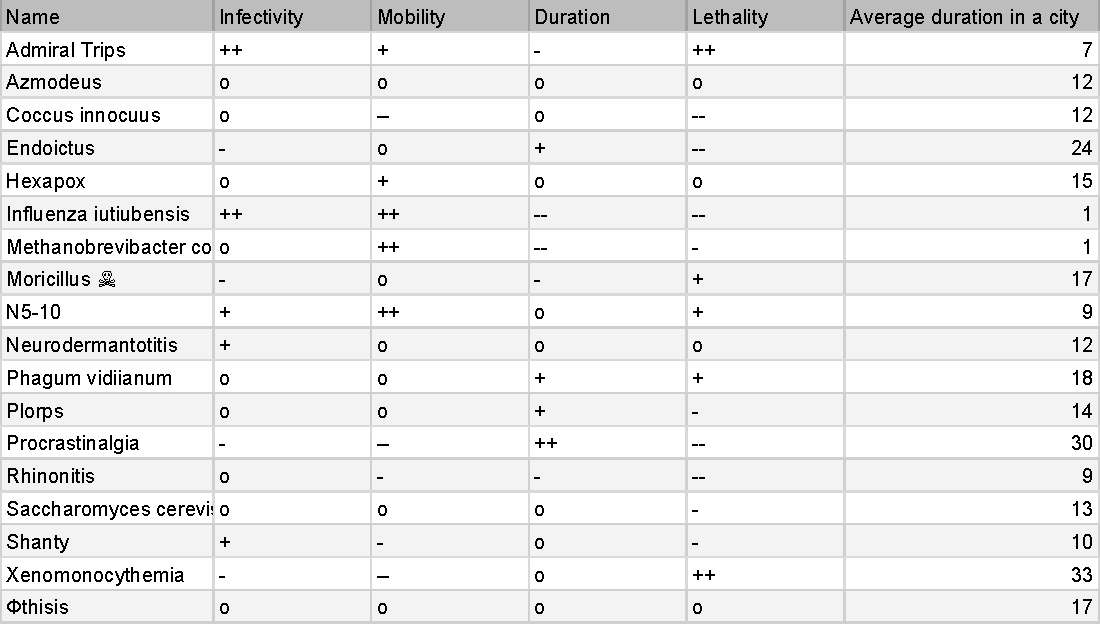
\includepdf[pages=-,pagecommand=\subsubsection{Pathogene}]{resources/pathogens.pdf}
\subsubsection{Städte}
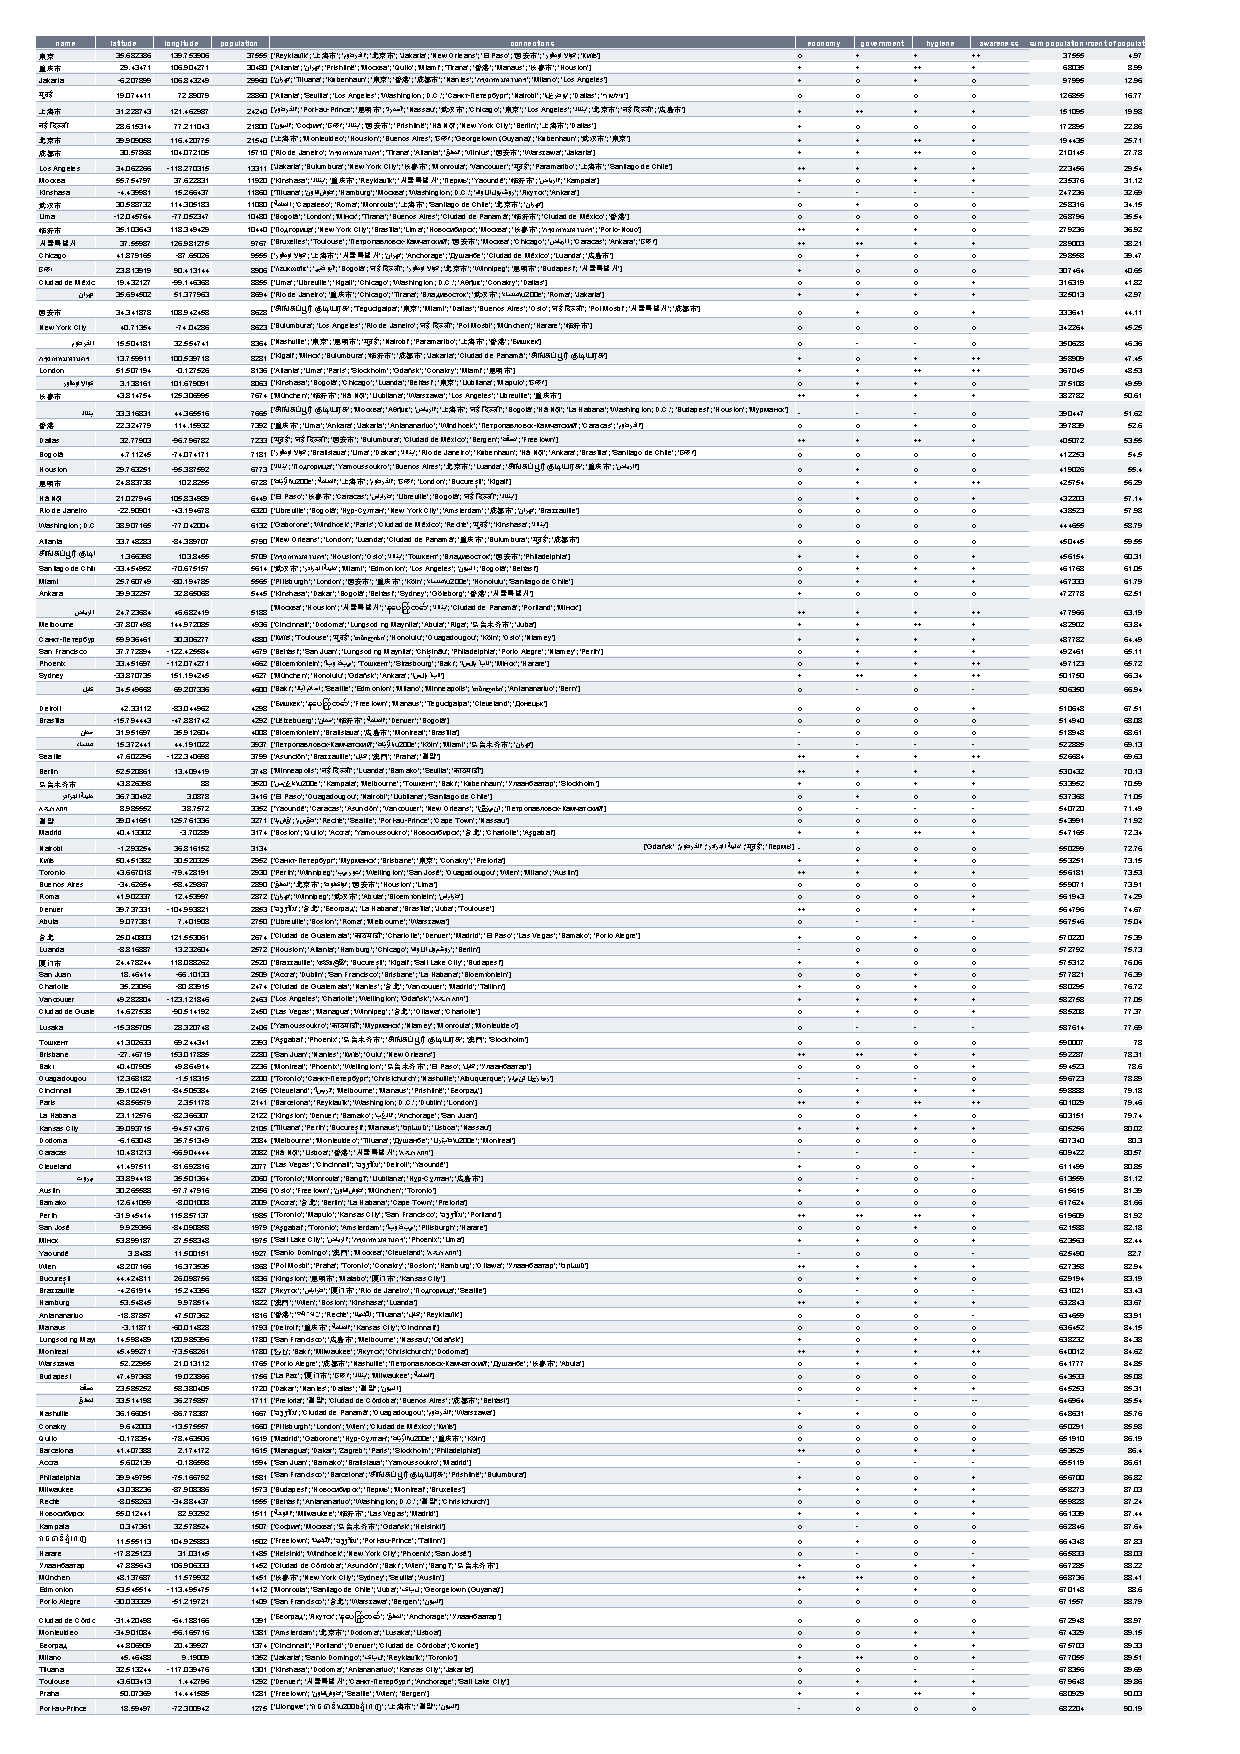
\includepdf[pages=-]{resources/cities.pdf}

\subsubsection{Seeds}
Die folgenden Seeds wurden nur mit der Aktion \gquote{Runde beenden} gespielt.
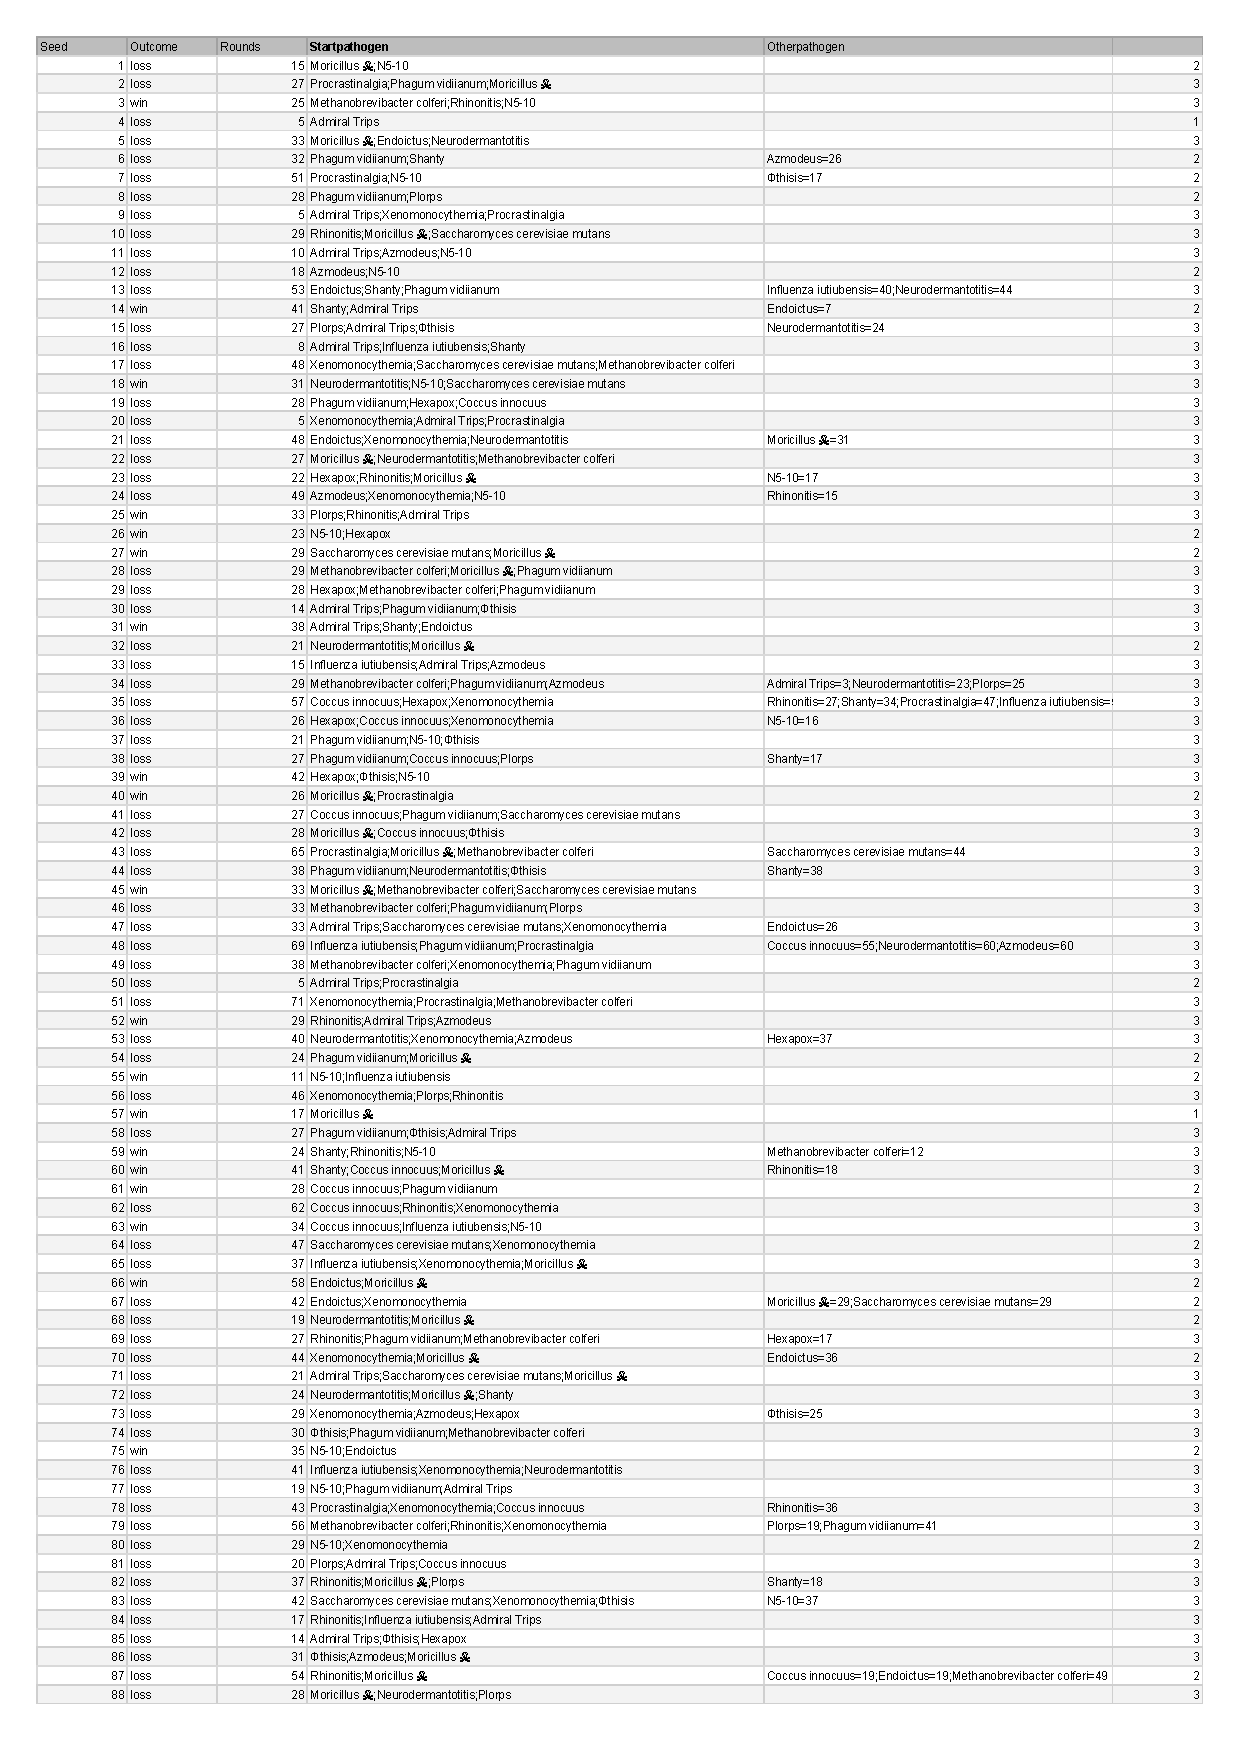
\includepdf[pages=-]{resources/seeds.pdf}

\subsubsection{Seeds mit Starteigenschaften}
\subsection{Wichtige Codeauszüge}
\label{sec:CodeErklaerung}
In diesem Kapitel werden essentielle Methoden, Codeauszüge und Klassen vorgestellt.
\label{code:IgnorePathogen}
\begin{lstlisting}[title=Methode die entscheidet ob es sich bei einem Pathogen um ein \gls{ignoriertes Pathogen} handelt oder nicht.]
public boolean ignorePathogenThisRound(Pathogen pathogen) {

    ...
    
    // Alle boolschen Werte zum Pruefen ob ein Pathogen ignoriert werden soll.
	boolean isOld = this.getRound() - encounter.get().getRound() >= 10;
	boolean hasLessAverage = this.getOutbreakEvents().stream().filter(e -> e.getPathogen() == pathogen)
			.mapToDouble(e -> e.getPrevalence()).average().orElseGet(() -> 0) <= 0.10;
	long numberOfCities = this.getOutbreakEvents().stream().filter(e -> e.getPathogen() == pathogen).count();
	boolean hasFewCities = numberOfCities <= 10;
	boolean hasNoCity = numberOfCities <= 0;

    // Sollten diese beiden boolschen Werte wahr sein, werden keine Pathogene ignoriert
	boolean enoughPoints = this.points <= 200;
	boolean hasVeryFewCities = this.getOutbreakEvents().stream().count() <= 5;
	if (enoughPoints && hasVeryFewCities) {
		return false;
	}

    // Pruefe ob ein das aktuelle Pathogen alle Eigenschaften zum ignorieren erfuellt. 
	boolean result = (isOld && (hasLessAverage || hasFewCities)) || hasNoCity;
	this.ignoredPathogens.put(pathogen, result);
	return result;
}
\end{lstlisting}
\label{code:ScaleErklaerung}
\begin{lstlisting}[title=Numerische Repräsentation der Werte von z.B. \gquote{Infectivity} eines Pathogens]
public int getValue() {
	switch (this) {
	case MM:    // Entspricht --
		return 1;
	case M:     // Entspricht -
		return 2;
	case N:     // Entspricht o
		return 3;
	case P:     // Entspricht +
		return 4;
	case PP:    // Entspricht ++
		return 5;
	}

	return 0;
}
\end{lstlisting}
\label{code:DoQuarantine}
\newpage
\begin{lstlisting}[title=Methode zum Entscheiden ob Pathogen unter Quarantäne gesetzt werden soll]
private static boolean doQuarantine(Pathogen pathogen) {

	int infectivity = pathogen.getInfectivity().getNumericRepresentation();
	int lethality = pathogen.getLethality().getNumericRepresentation();
	int mobility = pathogen.getMobility().getNumericRepresentation();
	int duration = pathogen.getDuration().getNumericRepresentation();

	// Factors that contribute to a dangerous pathogen killing lots of people in a
	// short amount of time
	// get multiplied. High duration would lead to a long and therefore expensive
	// Quaratine. Therefore we reverse the
	// scale of the duration.
	int score = infectivity * lethality * mobility * (6 - duration);

	return score >= constants.get("QUARANTINE_THRESHOLD");
}
\end{lstlisting}
\label{code:DoDevVaccine}
\begin{lstlisting}[title={Methode zum Entscheiden, ob Impfstoff entwickelt werden soll}]
private static boolean doDevVaccine(Pathogen pathogen) {

	int infectivity = pathogen.getInfectivity().getNumericRepresentation();
	int mobility = pathogen.getMobility().getNumericRepresentation();

	int score = mobility * infectivity;

	if (pathogen.getDuration() == Scale.MM) {
		return false;
	}

	if (doQuarantine(pathogen)) {
		return false;
	}

	// If a pathogen expands slowly, vaccines should be developed.
	return score <= constants.get("MAX_SLOW_PRODUCT");
}
\end{lstlisting}

\label{code:DoDevMedication}
\begin{lstlisting}[title={Methode zum Entscheiden, ob Medikament entwickelt werden soll}]
private static boolean doDevMedication(Pathogen pathogen) {

	int infectivity = pathogen.getInfectivity().getNumericRepresentation();
	int mobility = pathogen.getMobility().getNumericRepresentation();

	int score = mobility * infectivity;

	if (pathogen.getDuration() == Scale.MM) {
		return false;
	}

	// Because quarantine only contains a pathogen within one city it is not worth
	// the
	// points to develop a medication
	if (doQuarantine(pathogen)) {
		return false;
	}

	// If a pathogen expands fast, medication should be developed.
	return score > constants.get("MIN_FAST_PRODUCT");
}
\end{lstlisting}

\label{code:QuarantineForCity}
\begin{lstlisting}[title={Teil der Quarantäne Evaluation, welche bestimmt, ob die größte, uninfizierte Stadt vor mindestens zwei Ausbrüchen von starken Pathogenen geschützt werden muss}]
*
* If a very strong pathogen for instance Admiral Trips breaks out in two or
* more cities protect the biggest city.
*/
if (!city.isInfected()) {
	// Count outbreaks that would normaly require quarantine.
	long strongPathogenAmount = game.getOutbreakEvents().stream().filter(e -> doQuarantine(e.getPathogen()))
			.count();

	// If the counter is two or greater put the biggest city under quarantine
	if (strongPathogenAmount >= 2) {
		score += constants.get("QUARANTINE_FACTOR") * action.getRounds() * city.getPopulation();
		break;
	}
}
\end{lstlisting}

\label{code:QuarantineAtEnd}
\begin{lstlisting}[title={Teil der Quarantäne Evaluation, welche bestimmt, ob nur noch ein aktives Pathogen in einer Stadt existiert, welches sich nicht ausbreiten soll.}]
/*
 * Check if there is only one active one pathogen and if there is only one
 * outbreak event for this pathogen put it under quarantine (enclose a pathogen
 * inside a city).
 */
if (game.getPathEncounterEvents().stream().filter(e -> !game.ignorePathogenThisRound(e.getPathogen()))
		.count() == 1) {

	if (!city.isInfected()) {
		break;
	}

	// Safe the only pathogen as a variable as we will need it later two times.
	Pathogen onlyActivePathogen = game.getPathEncounterEvents().stream()
			.filter(e -> !game.ignorePathogenThisRound(e.getPathogen())).findAny().get().getPathogen();

	// Check that there is only one outbreak event for the only active pathogen and
	// that it is in the city for the current action.
	if ((game.getOutbreakEvents().stream().filter(e -> e.getPathogen() == onlyActivePathogen).count() == 1)
			&& city.isInfected(onlyActivePathogen)) {

		score += constants.get("QUARANTINE_FACTOR") * action.getRounds();
		break;
	}
}
\end{lstlisting}

\label{code:QuarantineForRest}
\begin{lstlisting}[title={Teil der Quarantäne Evaluation, welche bestimmt, ob der Rest der Welt vor dem Pathogen innerhalb einer Stadt geschützt werden muss.}]
// In a regular situation with no outbreak event a city does not require
// quarantine
if (!city.isInfected()) {
	break;
}

// Check if the pathogen in the city of the action needs to be quarantined
if (!doQuarantine(city.getPathogen())) {
	break;
}

// Check whether every city is infected and the quarantined pathogen can not
// spread any further. In this case there is no quarantine required.
if (game.getCities().stream().allMatch((City c) -> c.isInfected())) {
	break;
}

// City should be quarantine
score += constants.get("QUARANTINE_FACTOR") * action.getType().getCosts(action.getRounds());
break;
\end{lstlisting}
\newpage
\printglossary
\newpage
\noindent
\textbf{Eigenständigkeitserklärung} \\\\
\noindent
 Hiermit bestätigen wir, dass wir die vorliegende Arbeit selbständig verfasst und keine anderen als die angegebenen Hilfsmittel benutzt habe. Die Stellen der Arbeit, die dem Wortlaut oder dem Sinn nach anderen Werken (dazu zählen auch Internetquellen) entnommen sind, wurden unter Angabe der Quelle kenntlich gemacht. \\\\
 
\begin{center}
\line(1,0){350}
\end{center}
(Unterschriften, Datum)
 
\end{document}
